\section{Auswertung}
\label{sec:Auswertung}

Die Graphen werden sowohl mit Matplotlib \cite{matplotlib} als auch NumPy \cite{numpy} erstellt. Die Fehlerrechnung wird mithilfe von Uncertainties \cite{uncertainties} durchgeführt.

\subsection{Kalibrierung des Detektors}

\begin{figure}
	\centering
	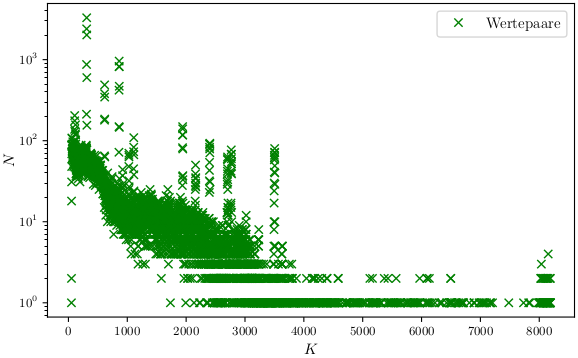
\includegraphics[width=\linewidth-70pt,height=\textheight-70pt,keepaspectratio]{content/images//EU152_1-8192.png}
	\caption{Das Spektrum eines $^{152}.{Eu}$-Strahlers, bei einer Messzeit von $\SI{2723}{\second}$, mit der Kanalnummer $K$ und der Anzahl der im Kanal nachgewiesenen Ereignisse $N$.}
	\label{fig:SpektrumEu}
\end{figure}

\begin{table}
	\centering
	\caption{Die Parameter der gefitteten Peaks des Spektrums von $^{152}.{Eu}$ mit den zugeordneten Energien.}
	\label{tab:a}
	\sisetup{table-format=1.2}
	\begin{tabular}{S[table-format=4.2]S[table-format=2.2]S[table-format=3.1]S[table-format=1.1]S[table-format=4.1]S[table-format=3.0]}
		\toprule
		{$E_\gamma^{\text{lit,\cite{MARTIN20131497}}}/\si{\kilo\electronvolt}$} & {$W^\text{\cite{MARTIN20131497}}/\si{\percent}$} & {$b$} & {$\sigma$} & {$a$} & {$c$} \\
		\midrule
		\SI{121.78\pm0.00} & \SI{28.53\pm0.18} & \SI{309.9\pm0.0} & \SI{1.1\pm0.0} & \SI{3213\pm  18} & \SI{68.1\pm5.2} \\
		\SI{244.70\pm0.00} & \SI{7.55\pm0.05} & \SI{615.0\pm0.0} & \SI{1.4\pm0.0} & \SI{ 455\pm   6} & \SI{24.5\pm2.0} \\
		\SI{295.94\pm0.00} & \SI{0.44\pm0.00} & \SI{741.7\pm0.2} & \SI{0.9\pm0.2} & \SI{  19\pm   3} & \SI{18.9\pm0.9} \\
		\SI{344.28\pm0.00} & \SI{26.59\pm0.21} & \SI{862.0\pm0.0} & \SI{1.6\pm0.0} & \SI{ 970\pm  13} & \SI{14.8\pm5.3} \\
		\SI{367.79\pm0.00} & \SI{0.86\pm0.01} & \SI{920.4\pm0.2} & \SI{1.8\pm0.2} & \SI{  28\pm   3} & \SI{11.2\pm1.3} \\
		\SI{411.12\pm0.00} & \SI{2.24\pm0.01} & \SI{1027.8\pm0.1} & \SI{1.7\pm0.1} & \SI{  59\pm   4} & \SI{12.2\pm1.9} \\
		\SI{443.96\pm0.00} & \SI{2.83\pm0.02} & \SI{1109.5\pm0.1} & \SI{1.7\pm0.1} & \SI{  88\pm   4} & \SI{10.8\pm1.8} \\
		\SI{688.67\pm0.01} & \SI{0.86\pm0.01} & \SI{1716.5\pm0.5} & \SI{3.0\pm0.6} & \SI{   9\pm   1} & \SI{8.8\pm0.7} \\
		\SI{778.90\pm0.00} & \SI{12.93\pm0.09} & \SI{1940.5\pm0.0} & \SI{2.1\pm0.1} & \SI{ 139\pm   3} & \SI{9.8\pm1.2} \\
		\SI{867.38\pm0.00} & \SI{4.23\pm0.03} & \SI{2160.3\pm0.3} & \SI{2.7\pm0.3} & \SI{  33\pm   3} & \SI{8.8\pm1.4} \\
		\SI{964.06\pm0.01} & \SI{14.51\pm0.08} & \SI{2400.0\pm0.1} & \SI{3.0\pm0.1} & \SI{  90\pm   3} & \SI{4.6\pm0.8} \\
		\SI{1005.27\pm0.05} & \SI{0.66\pm0.01} & \SI{2499.2\pm2.0} & \SI{8.6\pm4.9} & \SI{   3\pm   1} & \SI{2.5\pm1.4} \\
		\SI{1085.84\pm0.01} & \SI{10.11\pm0.06} & \SI{2702.6\pm0.2} & \SI{3.4\pm0.3} & \SI{  49\pm   3} & \SI{5.8\pm1.3} \\
		\SI{1112.08\pm0.00} & \SI{13.67\pm0.09} & \SI{2767.5\pm0.1} & \SI{3.4\pm0.1} & \SI{  69\pm   2} & \SI{2.7\pm0.7} \\
		\SI{1212.95\pm0.01} & \SI{1.41\pm0.01} & \SI{3017.8\pm0.5} & \SI{3.1\pm0.6} & \SI{   7\pm   1} & \SI{2.3\pm0.5} \\
		\SI{1299.14\pm0.01} & \SI{1.63\pm0.01} & \SI{3232.0\pm0.6} & \SI{4.4\pm0.7} & \SI{   5\pm   1} & \SI{0.7\pm0.2} \\
		\SI{1408.01\pm0.00} & \SI{20.87\pm0.11} & \SI{3502.4\pm0.1} & \SI{4.0\pm0.1} & \SI{  74\pm   1} & \SI{0.6\pm0.4} \\
		\SI{1457.64\pm0.01} & \SI{0.50\pm0.00} & \SI{3629.7\pm0.7} & \SI{6.1\pm0.8} & \SI{   3\pm   0} & \SI{0.3\pm0.1} \\
		\bottomrule
	\end{tabular}

	\label{tab:parameterEu}
\end{table}

\begin{figure}
	\centering
	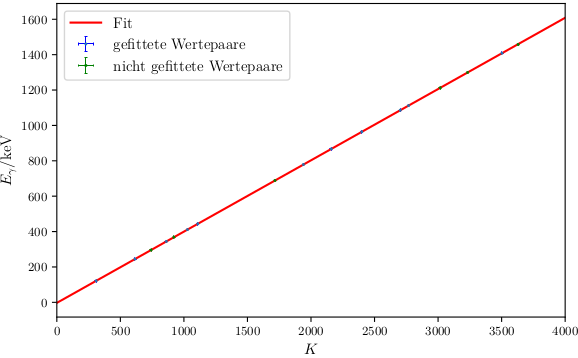
\includegraphics[width=\linewidth-70pt,height=\textheight-70pt,keepaspectratio]{content/images/EnergieKali.png}
	\caption{Die Energie $E_\gamma$ gegen die Kanalnummer $K$ aufgetragen, wobei die Unsicherheit des einzelnen Wertepaares sich durch die Unsicherheit der Position der Gaußkurve und der Unsicherheit des Literaturwertes für $E_\gamma$ ergibt.}
	\label{fig:Kalibrierungi}
\end{figure}

\subsection{Bestimmung der Effizienz des Detektors}

\begin{figure}
	\centering
	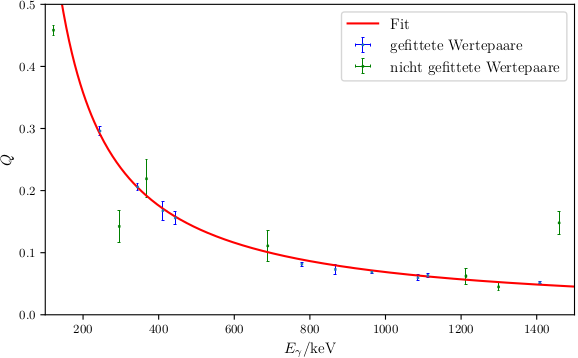
\includegraphics[width=\linewidth-70pt,height=\textheight-70pt,keepaspectratio]{content/images/Q.png}
	\caption{Die Vollenergienachweiswahrscheinlichkeit $Q$ gegen die Energie $E_\gamma$ aufgetragen.}
	\label{fig:Q}
\end{figure}

\begin{table}
	\centering
	\caption{Die berechneten Peakinhalte $Z$, die berechneten Vollenergienachweiswahrscheinlichkeiten $Q$, sowie die berechneten Energien $E_\gamma$. Zudem die aus der Literatur entnommenen Energien $E_\gamma^.{lit}$ und Emissions-Wahrscheinlichkeiten $W$.}
	\label{tab:a2}
	\sisetup{table-format=1.2}
	\begin{tabular}{S[table-format=4.2]S[table-format=4.2]S[table-format=2.2]S[table-format=5.0]S[table-format=0.3]}
		\toprule
		{$E_\gamma^{\text{lit,\cite{MARTIN20131497}}}/\si{\kilo\electronvolt}$} & {$E_\gamma$} & {$W^\text{\cite{MARTIN20131497}}/\si{\percent}$} & {$Z$} & {$Q$} \\
		\midrule
		\SI{121.78\pm0.00} & \SI{121.82\pm0.04} & \SI{28.53\pm0.18} & \SI{ 9030\pm   58} & \SI{0.458\pm0.008} \\
		\SI{244.70\pm0.00} & \SI{244.74\pm0.03} & \SI{7.55\pm0.05} & \SI{ 1543\pm   24} & \SI{0.296\pm0.007} \\
		\SI{295.94\pm0.00} & \SI{295.82\pm0.07} & \SI{0.44\pm0.00} & \SI{   43\pm    8} & \SI{0.142\pm0.026} \\
		\SI{344.28\pm0.00} & \SI{344.28\pm0.03} & \SI{26.59\pm0.21} & \SI{ 3779\pm   64} & \SI{0.206\pm0.005} \\
		\SI{367.79\pm0.00} & \SI{367.82\pm0.09} & \SI{0.86\pm0.01} & \SI{  130\pm   18} & \SI{0.219\pm0.031} \\
		\SI{411.12\pm0.00} & \SI{411.08\pm0.05} & \SI{2.24\pm0.01} & \SI{  259\pm   23} & \SI{0.168\pm0.015} \\
		\SI{443.96\pm0.00} & \SI{444.00\pm0.04} & \SI{2.83\pm0.02} & \SI{  304\pm   19} & \SI{0.156\pm0.010} \\
		\SI{688.67\pm0.01} & \SI{688.56\pm0.22} & \SI{0.86\pm0.01} & \SI{   66\pm   15} & \SI{0.111\pm0.025} \\
		\SI{778.90\pm0.00} & \SI{778.81\pm0.03} & \SI{12.93\pm0.09} & \SI{  727\pm   24} & \SI{0.081\pm0.003} \\
		\SI{867.38\pm0.00} & \SI{867.38\pm0.10} & \SI{4.23\pm0.03} & \SI{  213\pm   23} & \SI{0.073\pm0.008} \\
		\SI{964.06\pm0.01} & \SI{963.96\pm0.05} & \SI{14.51\pm0.08} & \SI{  687\pm   23} & \SI{0.069\pm0.003} \\
		\SI{1085.84\pm0.01} & \SI{1085.89\pm0.10} & \SI{10.11\pm0.06} & \SI{  417\pm   34} & \SI{0.060\pm0.005} \\
		\SI{1112.08\pm0.00} & \SI{1112.02\pm0.06} & \SI{13.67\pm0.09} & \SI{  597\pm   23} & \SI{0.063\pm0.003} \\
		\SI{1212.95\pm0.01} & \SI{1212.85\pm0.19} & \SI{1.41\pm0.01} & \SI{   61\pm   13} & \SI{0.062\pm0.013} \\
		\SI{1299.14\pm0.01} & \SI{1299.18\pm0.24} & \SI{1.63\pm0.01} & \SI{   51\pm    7} & \SI{0.045\pm0.007} \\
		\SI{1408.01\pm0.00} & \SI{1408.12\pm0.05} & \SI{20.87\pm0.11} & \SI{  744\pm   17} & \SI{0.052\pm0.001} \\
		\SI{1457.64\pm0.01} & \SI{1459.41\pm0.28} & \SI{0.50\pm0.00} & \SI{   51\pm    6} & \SI{0.148\pm0.019} \\
		\bottomrule
	\end{tabular}

	\label{tab:Q}
\end{table}

\subsection{Untersuchung des Spektrums von $^{137}.{Cs}$}

\begin{figure}
	\centering
	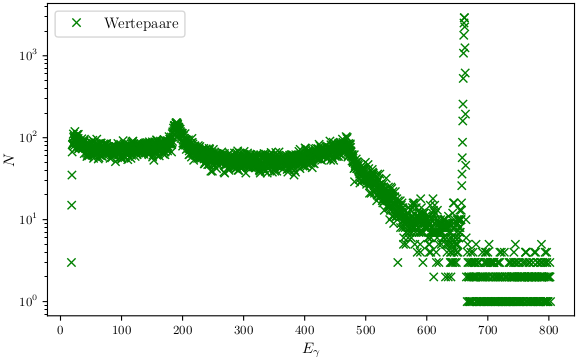
\includegraphics[width=\linewidth-70pt,height=\textheight-70pt,keepaspectratio]{content/images/Cs137.png}
	\caption{Das Spektrum eines $^{137}.{Cs}$-Strahlers, bei einer Messzeit von $\SI{4543}{\second}$.}
	\label{fig:SpektrumCs}
\end{figure}

\begin{table}
	\centering
	\caption{Die Parameter der gefitteten Peaks des Spektrums von $^{137}.{Cs}$ mit den ermittelten Energien, wobei es sich beim zweiten Peak um den Rückstreupeak handelt.}
	\label{tab:b}
	\sisetup{table-format=1.2}
	\begin{tabular}{S[table-format=4.4]@{${}\pm{}$}S[table-format=1.4]S[table-format=4.2]@{${}\pm{}$}S[table-format=1.2]S[table-format=1.2]@{${}\pm{}$}S[table-format=1.2]S[table-format=4.0]@{${}\pm{}$}S[table-format=2.0]S[table-format=2.1]@{${}\pm{}$}S[table-format=1.1]}
		\toprule
		\multicolumn{2}{c}{$E_\gamma/\si{\kilo\electronvolt}$} & \multicolumn{2}{c}{$b$} & \multicolumn{2}{c}{$\sigma$} & \multicolumn{2}{c}{$a$} & \multicolumn{2}{c}{$c$} \\
		\midrule
		661.4547 & 0.0241 & 1649.21 & 0.03 & 2.17 & 0.04 & 2983 & 39 & 20.3 & 15.8 \\
		190.8309 & 0.2637 & 481.17 & 0.65 & 14.50 & 0.75 &   63 &  3 & 77.9 & 1.2 \\
		\bottomrule
	\end{tabular}

	\label{tab:parameterCs}
\end{table}

\begin{figure}
	\centering
	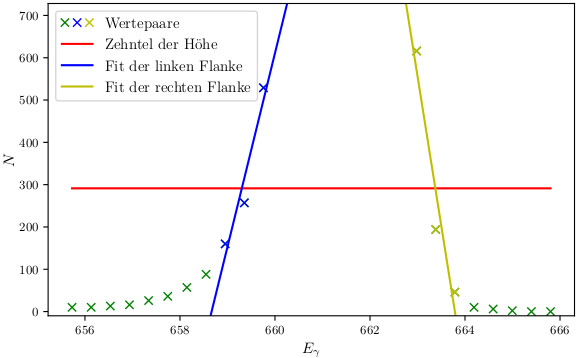
\includegraphics[width=\linewidth-70pt,height=\textheight-70pt,keepaspectratio]{content/images/Cs137Zehntel.png}
	\caption{Die Bestimmung der Zehntelwertsbreite des $^{137}.{Cs}$-Strahlers.}
	\label{fig:10tel}
\end{figure}

\begin{figure}
	\centering
	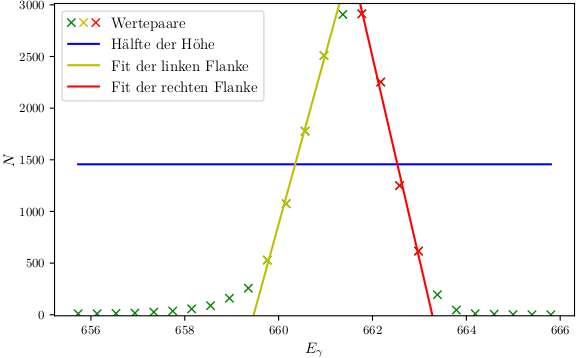
\includegraphics[width=\linewidth-70pt,height=\textheight-70pt,keepaspectratio]{content/images/Cs137Halb.png}
	\caption{Die Bestimmung der Halbwertsbreite des $^{137}.{Cs}$-Strahlers.}
	\label{fig:2tel}
\end{figure}

\begin{table}
	\centering
	\caption{Die Parameter der gefitteten Geraden zur Bestimmung der Halbwertsbreite und Zehntelbreite des Vollenergiepeaks des Spektrums von $^{137}.{Cs}$.}
	\label{tab:geraden1}
	\sisetup{table-format=1.2}
	\begin{tabular}{S[table-format=4.2]S[table-format=4.2]}
		\toprule
		{$a$} & {$b$} \\
		\midrule
		\SI{185\pm51} & \SI{-303003\pm83052} \\
		\SI{664\pm31} & \SI{-1092626\pm50811} \\
		\SI{-789\pm51} & \SI{1305453\pm83424} \\
		\SI{-285\pm79} & \SI{471675\pm130827} \\
		\bottomrule
	\end{tabular}

\end{table}

\begin{figure}
	\centering
	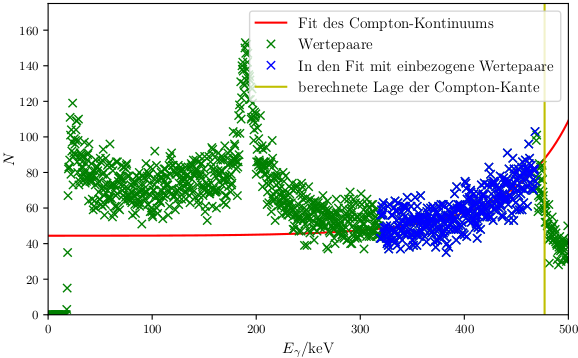
\includegraphics[width=\linewidth-70pt,height=\textheight-70pt,keepaspectratio]{content/images/Cs137Kon.png}
	\caption{Die Approximation des Compton-Kontinuums des $^{137}.{Cs}$-Strahlers.}
	\label{fig:Comptonkontinuum}
\end{figure}

\begin{figure}
	\centering
	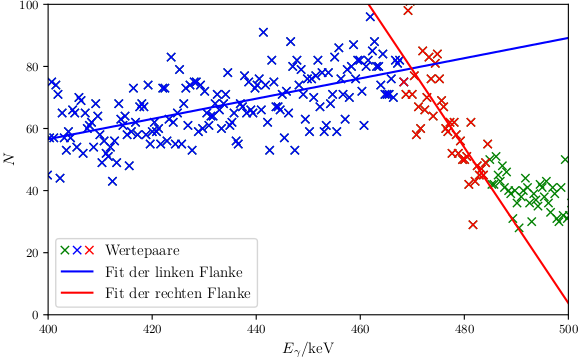
\includegraphics[width=\linewidth-70pt,height=\textheight-70pt,keepaspectratio]{content/images/Cs137Emax.png}
	\caption{Die Bestimmung der Position der Compton-Kante des $^{137}.{Cs}$-Strahlers.}
	\label{fig:Emax}
\end{figure}

\begin{table}
	\centering
	\caption{Die Parameter der gefitteten Geraden zur Bestimmung der Position der Compton-Kante des Spektrums von $^{137}.{Cs}$.}
	\label{tab:geraden2}
	\sisetup{table-format=1.2}
	\begin{tabular}{S[table-format=2.2]@{${}\pm{}$}S[table-format=1.2]S[table-format=4.0]@{${}\pm{}$}S[table-format=3.0]}
		\toprule
		\multicolumn{2}{c}{$m$} & \multicolumn{2}{c}{$n$} \\
		\midrule
		0.33 & 0.03 &  -74 &  14 \\
		-2.51 & 0.32 & 1257 & 151 \\
		\bottomrule
	\end{tabular}

\end{table}

\subsection{Bestimmung der Aktivität einer nicht eindeutig bestimmten Probe}

\begin{figure}
	\centering
	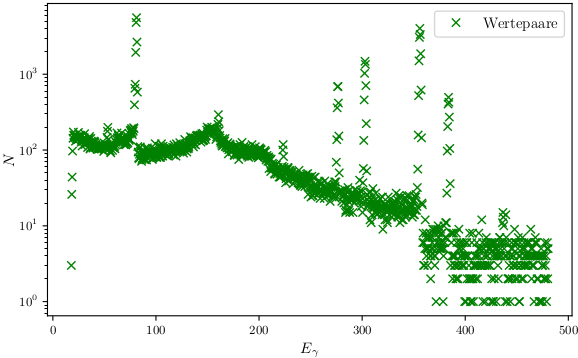
\includegraphics[width=\linewidth-70pt,height=\textheight-70pt,keepaspectratio]{content/images/D.png}
	\caption{Das Spektrum des Strahlers, bei einer Messzeit von $\SI{6312}{\second}$.}
	\label{fig:Ba}
\end{figure}

\begin{table}
	\centering
	\caption{Die Parameter der gefitteten Peaks des Spektrums mit den ermittelten Energien.}
	\label{tab:D}
	\sisetup{table-format=1.2}
	\begin{tabular}{S[table-format=3.2]@{${}\pm{}$}S[table-format=1.2]S[table-format=3.2]@{${}\pm{}$}S[table-format=1.2]S[table-format=1.2]@{${}\pm{}$}S[table-format=1.2]S[table-format=4.0]@{${}\pm{}$}S[table-format=3.0]S[table-format=3.1]@{${}\pm{}$}S[table-format=2.1]}
		\toprule
		\multicolumn{2}{c}{$E_\gamma/\si{\kilo\electronvolt}$} & \multicolumn{2}{c}{$b$} & \multicolumn{2}{c}{$\sigma$} & \multicolumn{2}{c}{$a$} & \multicolumn{2}{c}{$c$} \\
		\midrule
		81.02 & 0.05 & 208.63 & 0.04 & 1.06 & 0.04 & 5596 & 164 & 222.0 & 55.2 \\
		276.41 & 0.04 & 693.56 & 0.02 & 1.31 & 0.02 &  709 &   6 & 27.0 & 0.7 \\
		302.87 & 0.03 & 759.25 & 0.02 & 1.41 & 0.02 & 1501 &  11 & 22.7 & 3.5 \\
		356.00 & 0.03 & 891.11 & 0.01 & 1.51 & 0.01 & 4000 &  17 & 19.4 & 6.0 \\
		383.81 & 0.03 & 960.13 & 0.02 & 1.64 & 0.03 &  493 &   5 & 5.8 & 1.9 \\
		\bottomrule
	\end{tabular}

	\label{tab:parameterBa}
\end{table}

\begin{table}
	\centering
	\caption{Die berechneten Peakinhalte $Z$, die mit den Vollenergienachweiswahrscheinlichkeiten $Q$ berechneten Aktivitäten $A$,  sowie die berechneten Energien $E_\gamma$.  Zudem die aus der Literatur entnommenen Energien $E_\gamma^\text{lit}$ und Emissions-Wahrscheinlichkeiten $W$.}
	\label{tab:D2}
	\sisetup{table-format=1.2}
	\begin{tabular}{S[table-format=3.4]@{${}\pm{}$}S[table-format=1.4]S[table-format=3.2]@{${}\pm{}$}S[table-format=1.2]S[table-format=2.2]@{${}\pm{}$}S[table-format=1.2]S[table-format=5.0]@{${}\pm{}$}S[table-format=3.0]S[table-format=1.3]@{${}\pm{}$}S[table-format=1.3]S[table-format=4.0]@{${}\pm{}$}S[table-format=2.0]}
		\toprule
		\multicolumn{2}{c}{$E_\gamma^{\text{lit,\cite{KHAZOV2011855}}}/\si{\kilo\electronvolt}$} & \multicolumn{2}{c}{$E_\gamma/\si{\kilo\electronvolt}$} & \multicolumn{2}{c}{$W^\text{\cite{KHAZOV2011855}}/\si{\percent}$} & \multicolumn{2}{c}{$Z$} & \multicolumn{2}{c}{$Q$} & \multicolumn{2}{c}{$A/\si{\becquerel}$} \\
		\midrule
		80.9979 & 0.0011 & 81.02 & 0.05 & 32.95 & 0.33 & 14932 & 526 & 0.903 & 0.043 &  511 & 31 \\
		276.3989 & 0.0012 & 276.41 & 0.04 & 7.16 & 0.05 &  2329 &  18 & 0.257 & 0.006 & 1290 & 32 \\
		302.8508 & 0.0005 & 302.87 & 0.03 & 18.34 & 0.13 &  5294 &  43 & 0.234 & 0.005 & 1258 & 30 \\
		356.0129 & 0.0007 & 356.00 & 0.03 & 62.05 & 0.19 & 15093 &  78 & 0.198 & 0.004 & 1250 & 25 \\
		383.8485 & 0.0012 & 383.81 & 0.03 & 8.94 & 0.07 &  2024 &  26 & 0.183 & 0.004 & 1257 & 29 \\
		\bottomrule
	\end{tabular}

	\label{tab:ABa}
\end{table}

\subsection{Identifizierung der aktiven Nuklide in einer Zerfallsreihe}

\begin{figure}
	\centering
	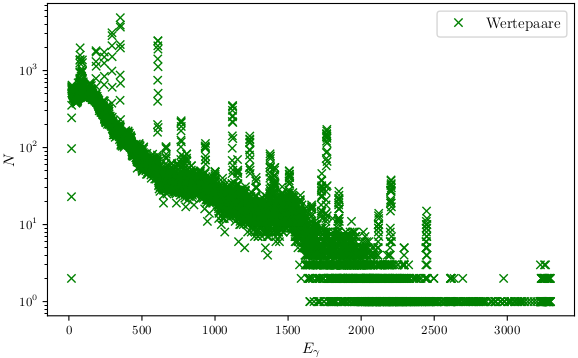
\includegraphics[width=\linewidth-70pt,height=\textheight-70pt,keepaspectratio]{content/images/unbekannt.png}
	\caption{Das aufgenommene Spektrum einer unbekannten Probe, bei einer Messzeit von $\SI{4489}{\second}$.}
	\label{fig:SpektrumUnbekannt}
\end{figure}

\begin{table}
	\centering
	\caption{Die Parameter der gefitteten Peaks des unbekannten Spektrums mit den ermittelten Energien.}
	\label{tab:unbekannt}
	\sisetup{table-format=1.2}
	\begin{tabular}{S[table-format=4.2]@{${}\pm{}$}S[table-format=1.2]S[table-format=4.2]@{${}\pm{}$}S[table-format=1.2]S[table-format=1.2]@{${}\pm{}$}S[table-format=1.2]S[table-format=4.0]@{${}\pm{}$}S[table-format=2.0]S[table-format=3.0]@{${}\pm{}$}S[table-format=2.0]}
		\toprule
		\multicolumn{2}{c}{$E_\gamma/\si{\kilo\electronvolt}$} & \multicolumn{2}{c}{$b$} & \multicolumn{2}{c}{$\sigma$} & \multicolumn{2}{c}{$a$} & \multicolumn{2}{c}{$c$} \\
		\midrule
		92.62 & 0.07 & 237.41 & 0.14 & 1.20 & 0.15 &  810 & 79 & 589 & 24 \\
		186.07 & 0.04 & 469.35 & 0.03 & 1.37 & 0.03 & 1449 & 24 & 423 &  8 \\
		242.01 & 0.04 & 608.18 & 0.03 & 1.31 & 0.03 & 1478 & 26 & 273 &  8 \\
		295.23 & 0.03 & 740.28 & 0.01 & 1.37 & 0.01 & 2982 & 18 & 194 &  6 \\
		351.90 & 0.03 & 880.92 & 0.02 & 1.50 & 0.02 & 4620 & 32 & 150 &  9 \\
		609.11 & 0.03 & 1519.30 & 0.03 & 2.09 & 0.03 & 2478 & 22 &  52 &  7 \\
		768.13 & 0.04 & 1913.96 & 0.08 & 2.54 & 0.09 &  188 &  5 &  36 &  2 \\
		933.90 & 0.07 & 2325.39 & 0.15 & 3.04 & 0.16 &   81 &  4 &  28 &  2 \\
		1120.07 & 0.04 & 2787.46 & 0.05 & 3.09 & 0.05 &  334 &  5 &  21 &  2 \\
		1377.49 & 0.11 & 3426.36 & 0.26 & 3.63 & 0.28 &   59 &  4 &  17 &  2 \\
		1401.45 & 0.14 & 3485.81 & 0.32 & 3.45 & 0.52 &   19 &  2 &  16 &  2 \\
		1508.87 & 0.13 & 3752.41 & 0.29 & 3.88 & 0.32 &   34 &  3 &  14 &  1 \\
		1729.46 & 0.11 & 4299.91 & 0.24 & 4.74 & 0.26 &   32 &  2 &   4 &  1 \\
		1764.27 & 0.08 & 4386.30 & 0.12 & 4.71 & 0.13 &  163 &  4 &   4 &  2 \\
		2203.97 & 0.12 & 5477.59 & 0.20 & 5.72 & 0.21 &   34 &  2 &   1 &  1 \\
		\bottomrule
	\end{tabular}

	\label{tab:parameterUnbekannt}
\end{table}

\begin{table}
	\centering
	\caption{Die berechneten Peakinhalte $Z$, die mit den Vollenergienachweiswahrscheinlichkeiten $Q$ berechneten Aktivitäten $A$, sowie die berechneten Energien $E_\gamma$. Zudem die aus der Literatur entnommenen Energien $E_\gamma^\text{lit}$ und Emissions-Wahrscheinlichkeiten $W$.}
	\label{tab:unbekannt2}
	\sisetup{table-format=1.2}
	\begin{tabular}{S[table-format=4.2]@{${}\pm{}$}S[table-format=1.2]S[table-format=4.0]S[table-format=2.0]}
		\toprule
		\multicolumn{2}{c}{$E_\gamma/\si{\kilo\electronvolt}$} & {$E_\gamma^{\text{lit}}/\si{\kilo\electronvolt}$} & {$W/\si{\percent}$} \\
		\midrule
		92.62 & 0.07 &   93 &  4 \\
		186.07 & 0.04 &  186 &  4 \\
		242.01 & 0.04 &  242 &  4 \\
		295.23 & 0.03 &  295 & 19 \\
		351.90 & 0.03 &  352 & 36 \\
		609.11 & 0.03 &  609 & 47 \\
		768.13 & 0.04 &  769 &  5 \\
		933.90 & 0.07 &  935 &  3 \\
		1120.07 & 0.04 & 1120 & 17 \\
		1377.49 & 0.11 & 1378 &  5 \\
		1401.45 & 0.14 & 1400 &  4 \\
		1508.87 & 0.13 & 1509 &  2 \\
		1729.46 & 0.11 & 1728 &  3 \\
		1764.27 & 0.08 & 1764 & 17 \\
		2203.97 & 0.12 & 2204 &  5 \\
		\bottomrule
	\end{tabular}

	\label{tab:AUnbekannt}
\end{table}

